\subsection{Äquidistante Zylinder Projektion}
\label{sec:aequizylinder} 
Die äquidistante Zylinder Projektion ist die einfachste Projektion. Sie stellt die Erde einfach in Längen- und Breitengrad dar. Dabei entsteht ein gleichmäßiges Gitterraster. Die Projektion ist weder winkel- noch flächentreu, das heißt, dass die Verzerrung mit der Entfernung vom Mittelpunkt der Karte zunimmt.\\ 
Vorteil der äquidistanten Zylinder Projektion:
\begin{itemize}
\item Die Projektion ist sehr einfach zu berechnen.
\end{itemize}
Nachteil der äquidistanten Zylinder Projektion:\\
\begin{itemize}
\item Die Verzerrungen wirken sowohl auf die Fläche als auch auf die Abstände aus.
\end{itemize}

Formel:\\
\begin{eqnarray*}
\cal{X} & = & \lambda\\
\cal{Y} & = & \varphi
\end{eqnarray*}

\begin{figure}[hbtp]
\centering
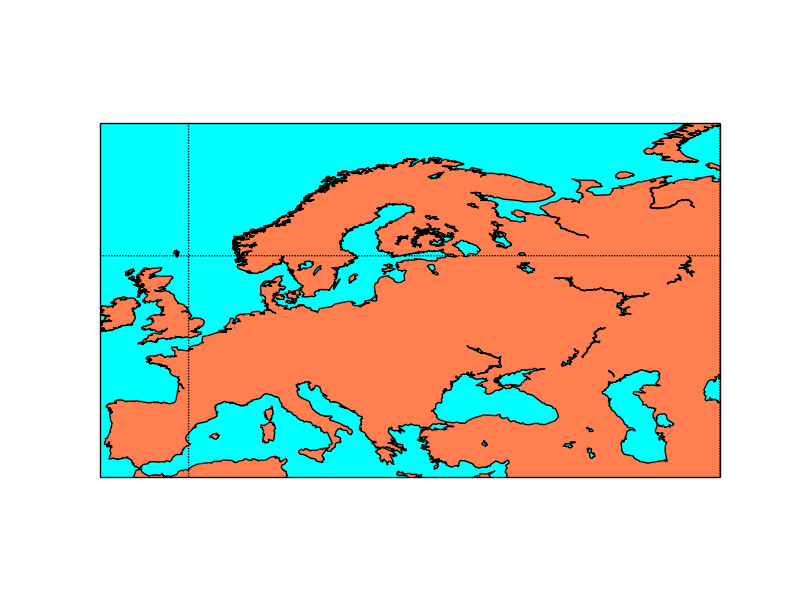
\includegraphics[scale=0.5,origin=c]{/Users/student/seminar/Kartendarstellungen/seminar/cyl}\\
\caption{Äquidistante Zylinderprojektion}
\end{figure}
 \newpage 